\subsection{Evaluation}
\label{sec:evaluation}

This section presents preliminary results for some of the implementations described in the previous section. In particular, the experiments focus on the speedup achieved by the {\sc bfs} and PageRank. The GPU implementations are compared against their multi-threaded CPU counterparts under synthetic and real-world graphs workloads. Table~\ref{tab:workload} summarizes the workloads\footnote{\url{http://snap.stanford.edu/data/}}. The Chain10K and Complete10K workloads are synthetic and represent a doubly linked chain and fully connected graphs, respectively.


\begin{table}[ht]
\centering
\begin{tabular}{l|r|r|c}
Name              & $|V|$   & $|E|$      & Directed \\\hline
Chain10K             & 10,000  & 9,999      & no       \\\hline
Complete10K          & 10,000  & 99,990,000 & no       \\\hline
Web (Google)      & 875,713 & 5,105,039  & yes      \\\hline
Web (NotreDame)   & 325,729 & 1,497,134  & yes      \\\hline
Web (Stanford)    & 281,903 & 2,312,497  & yes      \\\hline
OSN (LiveJournal) & 4,847,571 & 68,993,773 & yes    \\\hline
\end{tabular}
\caption{Graphs used in the experiments.}
\label{tab:workload}
\end{table}

We evaluate the implementation of the algorithms on a machine with dual-socket Intel Xeon Quad-core processor (E5520 @ 2.27GHz), and 16GB of system memory. The GPU installed on the machine is NVIDIA GeForce GTX 480: 480 cores clocked at 1400MHz, and has 1536 MB memory. We show the speedup of a multi-threaded CPU (using OpenMP) and GPU version compared to a single threaded CPU.

Figure \ref{fig:speedup:bfs} shows the speed up for BFS implementation. A chain is the structure that exhibits the worst opportunities for parallelism among the graphs since there is just one vertex per level. The Chain10K workload shows the results for this case, the OpenMP version achieves small speedup ($1.4x$) while the GPU version is $~3x$ slower than the sequential CPU version. The complete graph produces an unbalanced load among threads since most part of the work is performed by the first thread launched. It happens because the first thread, which is responsible for visiting the neighbors of the source vertex, has to visit all vertices in the graph. The OpenMP version achieves speedup of $4.4x$ and the GPU version performance is equivalent to the sequential CPU.

\begin{figure*}[htbp]
\begin{center}
\mbox{
\subfigure[BFS]
{\scalebox{0.425}{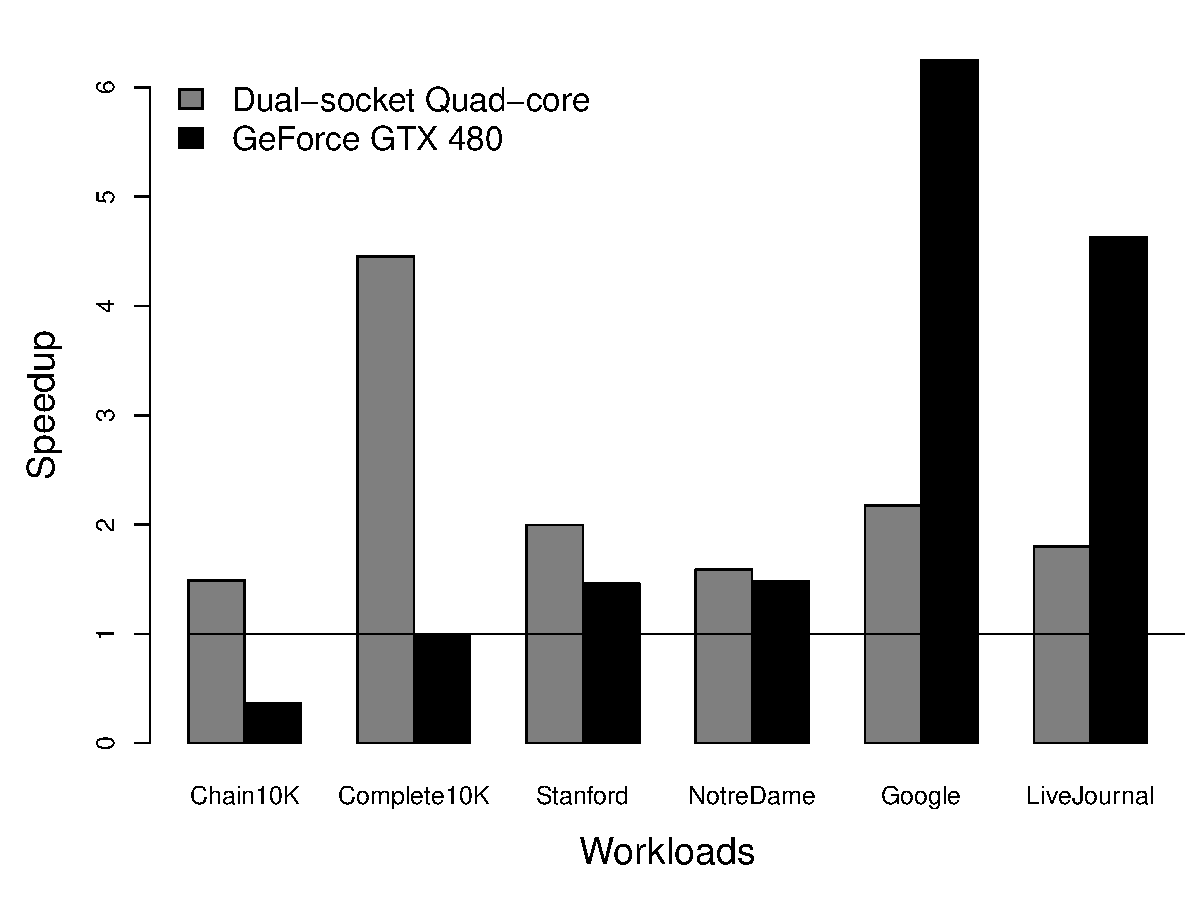
\includegraphics{figures/bfs}}
\label{fig:speedup:bfs}}
\subfigure[Page Rank]
{\scalebox{0.425}{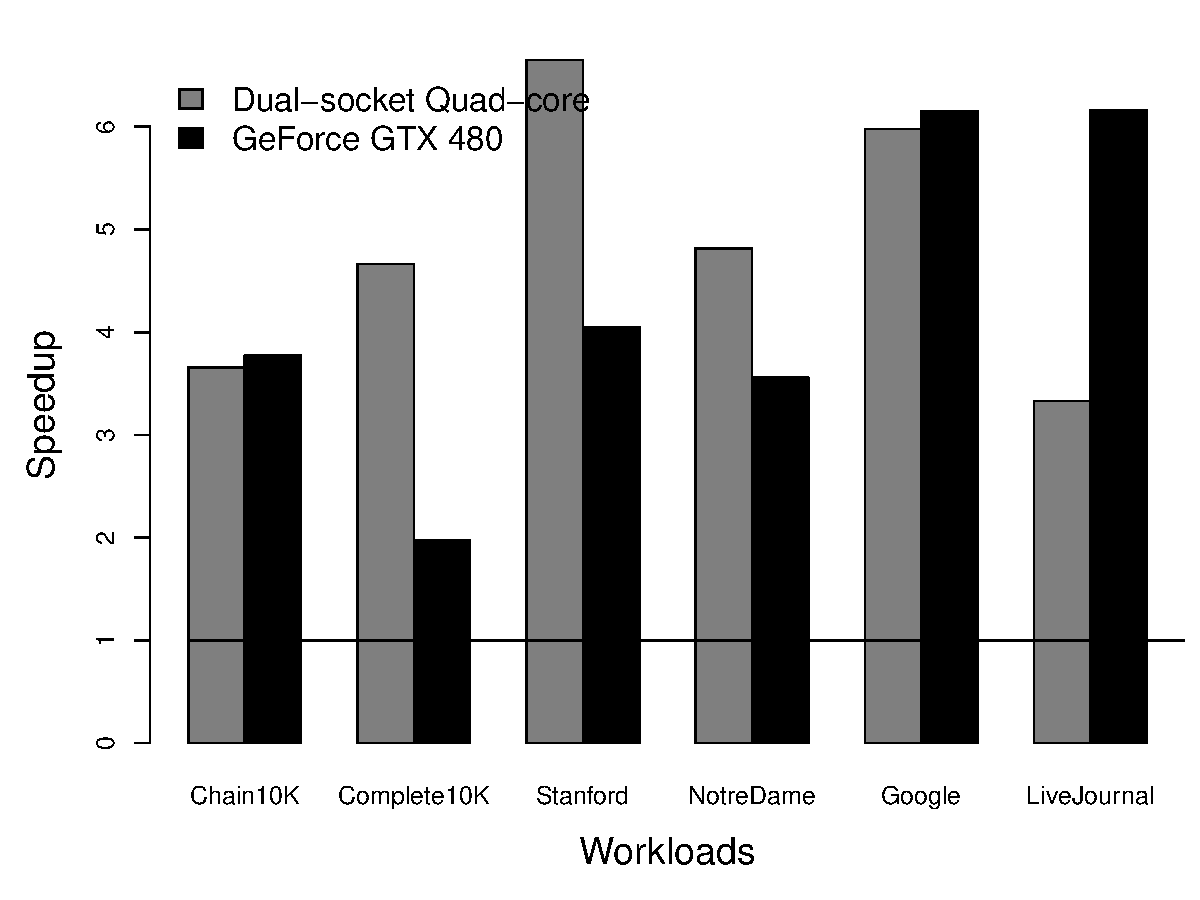
\includegraphics{figures/pagerank}}
\label{fig:speedup:pagerank}}
}
\caption{Performace results for BFS and PageRank}
\label{fig:speedup}
\end{center}
\end{figure*}

Figure \ref{fig:speedup:pagerank} shows the results for the PageRank algorithm. For the Chain10K workload, both OpenMP and GPU versions achieve $~3.6x$ speedup. Not shown in the figure, because the graph is relatively small, half of the GPU time is spent on data transfers as it is dominated by the channel's latency. If we consider only the kernel time, the GPU version achieves over $7x$ speedup (i.e., $2x$ compared to OpenMP).

For the Complete10K workload, in each round, each vertex accesses the rank of each other vertex. The OpenMP version achieves over $4.5x$ speedup; however the GPU version only achieves $~2x$ speedup. Although all threads have the same amount of workload, we expect that threads access the same memory location in every step reduces memory access bandwidth for the GPU, however a better investigation of why we get this result is due.

The chain and complete graphs are good workloads to understand the performance of GPU version in extreme cases of graph connectedness. However, they are not the typical case for most part of the applications. For the other workloads, based on real-world graphs, the results for BFS and Page Rank implementations are similar. The amount of vertices and connectedness of these graphs give a better opportunity to use the GPU resources. The distribution of neighbors of the vertices gives reasonable amount of work per thread and also balances the load among threads.
